\subsubsection{Reusability and modifiability} \label{section:reuse}
Blockchain applications are typically easy to deploy, reuse and modify, as long as the contract-oriented language Solidity allows it. Deployment of additional services on smart contracts is a relatively easy process. Usage of an API is desired in the centralized systems, as it increases the quality reusability and modifiability quality attributes.

\paragraph{Connecting multiple platforms to DApps}
Once a DApp is deployed onto the chain, it, if implemented properly, can be used as a core foundation for a platform with similar purpose. Multiple platforms can be connected to the same DApp in the same way as multiple DApps are connected to the Ethereum network. Individual smart contracts do not have any defined maximum throughput, thus, increased transaction density, that targets a specific smart contract, does not degrade its performance (more specific details on that topic can be found in \ref{section:scalability}). There is as well no need for any additional hardware components in case of increased traffic, as it is with centralized systems.

\paragraph{Modifying and reusing centralized applications}
Centralized applications' reusability and modifiability is highly dependent on the quality of implementation. Usage of design patterns that improve the code's reusability and modifiability is highly beneficial, in case of those quality attributes being important for a particular system. Typical design patterns, that are used for that purpose, are the Adapter and Facade design patterns.

In client-server applications, a good way to improve a system's reusability, modifiability and scalability is to implement an application programming interface (API), that handles the communication between the client side (frontend) and the server side (backend). In other words, API's task is to connect various components of the application. Usage of an API for component communication follows the guidelines for Facade design pattern. An example of that is illustrated in Figure \ref{fig:apipattern}.

\begin{figure}[H]
\centering
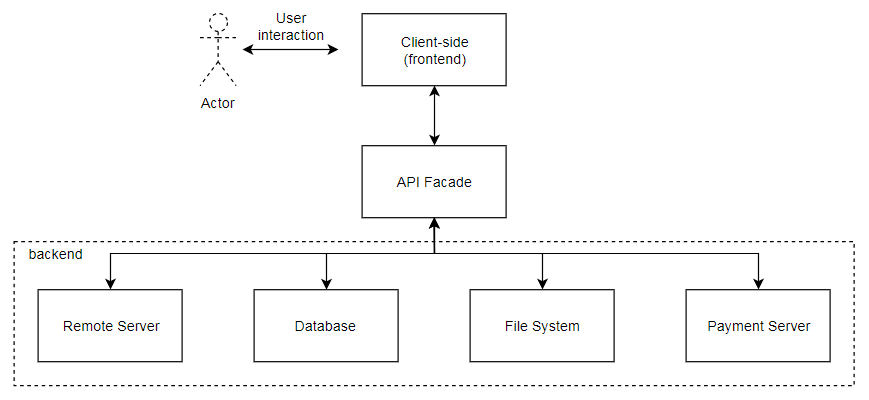
\includegraphics[scale=0.59]{images/facadeapi.png}
\caption{Illustration of API Facade design pattern.}
\label{fig:apipattern}
\end{figure}

Usage of an API as a hub for communication, results in individual components of the system being independent of eachother. Thus, different parts of the system can easily be modified or replaced, when needed, without affecting other parts of the system. 

APIs are, in some cases, used to introduce the functionality of integrating applications to other services. For example, Google Maps application has an API, which can be integrated into other web applications.

\paragraph{Modifying smart contracts and DApps}
As Ethereum is completely transparent, all source code of deployed smart contracts is available to the public. This follows the same ideology as most of the open-source software, namely that users have a freedom of extending and modifying the code in a way that they would like to. 

Many DApps, including the decentralized version of Secure Package adopt a token payment system by the customized ERC20 tokens. As all of the ERC20 tokens have to follow a specific standard, that is defined by the interface contract in Figure \ref{fig:erc20interface}, it is very easy to modify the existing payment system by deploying a contract, that follows that interface.

\begin{figure}[H]
\centering
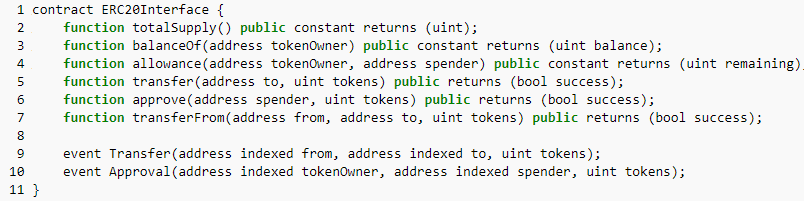
\includegraphics[scale=0.69]{images/erc20.png}
\caption{ERC20 interface contract \textnormal{\citep{erc20}}.}
\label{fig:erc20interface}
\end{figure}